%
% $Id: SANDExampleReportNotstrict.tex,v 1.26 2009/05/01 20:59:19 rolf Exp $
%
% This is an example LaTeX file which uses the SANDreport class file.
% It shows how a SAND report should be formatted, what sections and
% elements it should contain, and how to use the SANDreport class.
% It uses the LaTeX report class, but not the strict option.
%
% Get the latest version of the class file and more at
%    http://www.cs.sandia.gov/~rolf/SANDreport
%
% This file and the SANDreport.cls file are based on information
% contained in "Guide to Preparing {SAND} Reports", Sand98-0730, edited
% by Tamara K. Locke, and the newer "Guide to Preparing SAND Reports and
% Other Communication Products", SAND2002-2068P.
% Please send corrections and suggestions for improvements to
% Rolf Riesen, Org. 9223, MS 1110, rolf@cs.sandia.gov
%
%
\documentclass[pdf,12pt,report]{SANDreport}
\usepackage[light,first,bottomafter]{draftcopy}
\usepackage{algorithmic}
\usepackage{algorithm}
\usepackage{alltt}
\usepackage{amsbsy}
\usepackage{amscd}
\usepackage{amsfonts}
\usepackage{amsmath}
\usepackage{amssymb}
\usepackage{amsthm}
\usepackage{booktabs}
\usepackage{epsfig}
\usepackage{euscript}
\usepackage{fancyhdr}
\usepackage{float}
\usepackage{fullpage}
\usepackage{graphicx}
\usepackage{ifthen}
\usepackage{multirow}
\usepackage{supertabular}
\usepackage{times}
\usepackage{verbatim}
\usepackage{xfrac}
\usepackage{xspace}
\usepackage[colorlinks]{hyperref}
\usepackage[numbers,sort&compress]{natbib}
\usepackage[FIGBOTCAP,TABTOPCAP,bf,tight]{subfigure}
\usepackage[normalem]{ulem}

\usepackage[T1]{fontenc}
\usepackage{ae,aecompl}

\numberwithin{algorithm}{chapter}
%%%%%%%%%%%%%%%%%%%%%%%%%%%%%%%%%%%%%%%%%%%%%%%%%%%%%%%%%%%%%%%%%%%%%%%%
% editing
%%%%%%%%%%%%%%%%%%%%%%%%%%%%%%%%%%%%%%%%%%%%%%%%%%%%%%%%%%%%%%%%%%%%%%%%
%\usepackage[usenames,dvipsnames]{xcolor}
%\newcommand{\comment}[1]{\textcolor{blue}{[ \sc{#1} ]}} % comments
%\newcommand{\revise}[1]{\textcolor{red}{{#1}}} % revisions

%%%%%%%%%%%%%%%%%%%%%%%%%%%%%%%%%%%%%%%%%%%%%%%%%%%%%%%%%%%%%%%%%%%%%%%%
% abbreviations
%%%%%%%%%%%%%%%%%%%%%%%%%%%%%%%%%%%%%%%%%%%%%%%%%%%%%%%%%%%%%%%%%%%%%%%%
\newcommand{\aref}[1]{{App.~\ref{#1}}}
\newcommand{\eref}[1]{{Eq.~(\ref{#1})}}
\newcommand{\cref}[1]{{Ref.~\cite{#1}}}
\newcommand{\sref}[1]{{Sec.~\ref{#1}}}
\newcommand{\fref}[1]{{Fig.~\ref{#1}}}
\newcommand{\tref}[1]{{Table~\ref{#1}}}
\newcommand{\cf}{{cf.\,}}
\newcommand{\ie}{{i.e.\,}}
\newcommand{\vs}{{vs.\,}}
\newcommand{\eg}{{e.g.\,}}
\newcommand{\etal}{{et al.\,}}

%%%%%%%%%%%%%%%%%%%%%%%%%%%%%%%%%%%%%%%%%%%%%%%%%%%%%%%%%%%%%%%%%%%%%%%%
% tensors
%%%%%%%%%%%%%%%%%%%%%%%%%%%%%%%%%%%%%%%%%%%%%%%%%%%%%%%%%%%%%%%%%%%%%%%%
\renewcommand{\vec}[1]{{\boldsymbol{#1}}}
\newcommand{\chib}{\vec{\chi}}

%% suffix
\newcommand{\ab}{\vec{a}}
%\newcommand{\bb}{\vec{b}}
\newcommand{\vb}{\vec{v}}
\newcommand{\Ab}{\vec{A}}
\newcommand{\Bb}{\vec{B}}
\newcommand{\Tb}{\vec{T}}

%% prefix
\newcommand{\bzero}{\vec{0}}
\newcommand{\bone}{\vec{1}}

\newcommand{\bA}{\vec{A}}
\newcommand{\bB}{\vec{B}}
\newcommand{\bC}{\vec{C}}
\newcommand{\bD}{\vec{D}}
\newcommand{\bE}{\vec{E}}
\newcommand{\bF}{\vec{F}}
\newcommand{\bG}{\vec{G}}
\newcommand{\bH}{\vec{H}}
\newcommand{\bI}{\vec{I}}
\newcommand{\bJ}{\vec{J}}
\newcommand{\bK}{\vec{K}}
\newcommand{\bL}{\vec{L}}
\newcommand{\bM}{\vec{M}}
\newcommand{\bN}{\vec{N}}
\newcommand{\bO}{\vec{O}}
\newcommand{\bP}{\vec{P}}
\newcommand{\bQ}{\vec{Q}}
\newcommand{\bR}{\vec{R}}
\newcommand{\bS}{\vec{S}}
\newcommand{\bT}{\vec{T}}
\newcommand{\bU}{\vec{U}}
\newcommand{\bV}{\vec{V}}
\newcommand{\bW}{\vec{W}}
\newcommand{\bX}{\vec{X}}
\newcommand{\bY}{\vec{Y}}
\newcommand{\bZ}{\vec{Z}}

\newcommand{\ba}{\vec{a}}
\newcommand{\bb}{\vec{b}}
\newcommand{\bc}{\vec{c}}
\newcommand{\bd}{\vec{d}}
\newcommand{\be}{\vec{e}}
%\renewcommand{\bf}{\vec{f}}
\newcommand{\bff}{\vec{f}}
\newcommand{\bg}{\vec{g}}
\newcommand{\bh}{\vec{h}}
\newcommand{\bi}{\vec{i}}
\newcommand{\bj}{\vec{j}}
\newcommand{\bk}{\vec{k}}
\newcommand{\bl}{\vec{l}}
\newcommand{\bm}{\vec{m}}
\newcommand{\bn}{\vec{n}}
\newcommand{\bo}{\vec{o}}
\newcommand{\bp}{\vec{p}}
\newcommand{\bq}{\vec{q}}
\newcommand{\br}{\vec{r}}
\newcommand{\bs}{\vec{s}}
\newcommand{\bt}{\vec{t}}
\newcommand{\bu}{\vec{u}}
\newcommand{\bv}{\vec{v}}
\newcommand{\bw}{\vec{w}}
\newcommand{\bx}{\vec{x}}
\newcommand{\by}{\vec{y}}
\newcommand{\bz}{\vec{z}}

\newcommand{\balpha}{\vec{\alpha}}
\newcommand{\bbeta}{\vec{\beta}}
\newcommand{\bgamma}{\vec{\gamma}}
\newcommand{\bdelta}{\vec{\delta}}
\newcommand{\bepsilon}{\vec{\epsilon}}
\newcommand{\bvarepsilon}{\vec{\varepsilon}}
\newcommand{\bzeta}{\vec{\zeta}}
\newcommand{\beeta}{\vec{\eta}}
\newcommand{\btheta}{\vec{\theta}}
\newcommand{\bvartheta}{\vec{\vartheta}}
\newcommand{\bkappa}{\vec{\kappa}}
\newcommand{\blambda}{\vec{\lambda}}
\newcommand{\bmu}{\vec{\mu}}
\newcommand{\bnu}{\vec{\nu}}
\newcommand{\bxi}{\vec{\xi}}
\newcommand{\bomicron}{\vec{o}}
\newcommand{\bpi}{\vec{\pi}}
\newcommand{\bvarpi}{\vec{\varpi}}
\newcommand{\brho}{\vec{\rho}}
\newcommand{\bvarrho}{\vec{\varrho}}
\newcommand{\bsigma}{\vec{\sigma}}
\newcommand{\bvarsigma}{\vec{\varsigma}}
\newcommand{\btau}{\vec{\tau}}
\newcommand{\bupsilon}{\vec{\upsilon}}
\newcommand{\bphi}{\vec{\phi}}
\newcommand{\bvarphi}{\vec{\varphi}}
\newcommand{\bchi}{\vec{\chi}}
\newcommand{\bpsi}{\vec{\psi}}
\newcommand{\bomega}{\vec{\omega}}

\newcommand{\bGamma}{\vec{\Gamma}}
\newcommand{\bDelta}{\vec{\Delta}}
\newcommand{\bTheta}{\vec{\Theta}}
\newcommand{\bLambda}{\vec{\Lambda}}
\newcommand{\bXi}{\vec{\Xi}}
\newcommand{\bPi}{\vec{\Pi}}
\newcommand{\bSigma}{\vec{\Sigma}}
\newcommand{\bUpsilon}{\vec{\Upsilon}}
\newcommand{\bPhi}{\vec{\Phi}}
\newcommand{\bPsi}{\vec{\Psi}}
\newcommand{\bOmega}{\vec{\Omega}}

%%%%%%%%%%%%%%%%%%%%%%%%%%%%%%%%%%%%%%%%%%%%%%%%%%%%%%%%%%%%%%%%%%%%%%%%
% matrix
%%%%%%%%%%%%%%%%%%%%%%%%%%%%%%%%%%%%%%%%%%%%%%%%%%%%%%%%%%%%%%%%%%%%%%%%
\newcommand{\mat}[1]{\mathsf{#1}}
\newcommand{\transpose}[1]{{#1}^{\text{T}}}
\newcommand{\conjtransla}[1]{{#1}^{\text{*}}}
\newcommand{\conjtransqm}[1]{{#1}^{\dagger}}

%% suffix
\newcommand{\ws}{\mat{w}}
\newcommand{\As}{\mat{A}}
\newcommand{\Ms}{\mat{M}}

%% prefix
\newcommand{\szero}{\mat{0}}
\newcommand{\sone}{\mat{1}}

\newcommand{\sA}{\mat{A}}
\newcommand{\sB}{\mat{B}}
\newcommand{\sC}{\mat{C}}
\newcommand{\sD}{\mat{D}}
\newcommand{\sE}{\mat{E}}
\newcommand{\sF}{\mat{F}}
\newcommand{\sG}{\mat{G}}
\newcommand{\sH}{\mat{H}}
\newcommand{\sI}{\mat{I}}
\newcommand{\sJ}{\mat{J}}
\newcommand{\sK}{\mat{K}}
\newcommand{\sL}{\mat{L}}
\newcommand{\sM}{\mat{M}}
\newcommand{\sN}{\mat{N}}
\newcommand{\sO}{\mat{O}}
\newcommand{\sP}{\mat{P}}
\newcommand{\sQ}{\mat{Q}}
\newcommand{\sR}{\mat{R}}
\newcommand{\sS}{\mat{S}}
\newcommand{\sT}{\mat{T}}
\newcommand{\sU}{\mat{U}}
\newcommand{\sV}{\mat{V}}
\newcommand{\sW}{\mat{W}}
\newcommand{\sX}{\mat{X}}
\newcommand{\sY}{\mat{Y}}
\newcommand{\sZ}{\mat{Z}}

\newcommand{\sa}{\mat{a}}
\renewcommand{\sb}{\mat{b}}
\renewcommand{\sc}{\mat{c}}
\newcommand{\sd}{\mat{d}}
\newcommand{\se}{\mat{e}}
\renewcommand{\sf}{\mat{f}}
\newcommand{\sg}{\mat{g}}
\newcommand{\sh}{\mat{h}}
\newcommand{\si}{\mat{i}}
\newcommand{\sj}{\mat{j}}
\newcommand{\sk}{\mat{k}}
\renewcommand{\sl}{\mat{l}}
\newcommand{\sm}{\mat{m}}
\newcommand{\sn}{\mat{n}}
\newcommand{\so}{\mat{o}}
\renewcommand{\sp}{\mat{p}}
\newcommand{\sq}{\mat{q}}
\newcommand{\sr}{\mat{r}}
\renewcommand{\ss}{\mat{s}}
\newcommand{\st}{\mat{t}}
\newcommand{\su}{\mat{u}}
\newcommand{\sv}{\mat{v}}
\newcommand{\sw}{\mat{w}}
\newcommand{\sx}{\mat{x}}
\newcommand{\sy}{\mat{y}}
\newcommand{\sz}{\mat{z}}

\newcommand{\salpha}{\mat{\alpha}}
\newcommand{\sbeta}{\mat{\seta}}
\newcommand{\sgamma}{\mat{\gamma}}
\newcommand{\sdelta}{\mat{\delta}}
\newcommand{\sepsilon}{\mat{\epsilon}}
\newcommand{\svarepsilon}{\mat{\varepsilon}}
\newcommand{\szeta}{\mat{\zeta}}
\newcommand{\seta}{\mat{\eta}}
\newcommand{\stheta}{\mat{\theta}}
\newcommand{\svartheta}{\mat{\vartheta}}
\newcommand{\skappa}{\mat{\kappa}}
\newcommand{\slambda}{\mat{\lambda}}
\newcommand{\smu}{\mat{\mu}}
\newcommand{\snu}{\mat{\nu}}
\newcommand{\sxi}{\mat{\xi}}
\newcommand{\somicron}{\mat{o}}
\newcommand{\spi}{\mat{\pi}}
\newcommand{\svarpi}{\mat{\varpi}}
\newcommand{\srho}{\mat{\rho}}
\newcommand{\svarrho}{\mat{\varrho}}
\newcommand{\ssigma}{\mat{\sigma}}
\newcommand{\svarsigma}{\mat{\varsigma}}
\newcommand{\stau}{\mat{\tau}}
\newcommand{\supsilon}{\mat{\upsilon}}
\newcommand{\sphi}{\mat{\phi}}
\newcommand{\svarphi}{\mat{\varphi}}
\newcommand{\schi}{\mat{\chi}}
\newcommand{\spsi}{\mat{\psi}}
\newcommand{\somega}{\mat{\omega}}

\newcommand{\sGamma}{\mat{\Gamma}}
\newcommand{\sDelta}{\mat{\Delta}}
\newcommand{\sTheta}{\mat{\Theta}}
\newcommand{\sLambda}{\mat{\Lambda}}
\newcommand{\sXi}{\mat{\Xi}}
\newcommand{\sPi}{\mat{\Pi}}
\newcommand{\sSigma}{\mat{\Sigma}}
\newcommand{\sUpsilon}{\mat{\Upsilon}}
\newcommand{\sPhi}{\mat{\Phi}}
\newcommand{\sPsi}{\mat{\Psi}}
\newcommand{\sOmega}{\mat{\Omega}}

%%%%%%%%%%%%%%%%%%%%%%%%%%%%%%%%%%%%%%%%%%%%%%%%%%%%%%%%%%%%%%%%%%%%%%%%
% fourth-order tensors, common number sets
% latin/roman symbols only for now
%%%%%%%%%%%%%%%%%%%%%%%%%%%%%%%%%%%%%%%%%%%%%%%%%%%%%%%%%%%%%%%%%%%%%%%%

%% suffix

%% prefix
\newcommand{\bbA}{\mathbb{A}}
\newcommand{\bbB}{\mathbb{B}}
\newcommand{\bbC}{\mathbb{C}}
\newcommand{\bbD}{\mathbb{D}}
\newcommand{\bbE}{\mathbb{E}}
\newcommand{\bbF}{\mathbb{F}}
\newcommand{\bbG}{\mathbb{G}}
\newcommand{\bbH}{\mathbb{H}}
\newcommand{\bbI}{\mathbb{I}}
\newcommand{\bbJ}{\mathbb{J}}
\newcommand{\bbK}{\mathbb{K}}
\newcommand{\bbL}{\mathbb{L}}
\newcommand{\bbM}{\mathbb{M}}
\newcommand{\bbN}{\mathbb{N}}
\newcommand{\bbO}{\mathbb{O}}
\newcommand{\bbP}{\mathbb{P}}
\newcommand{\bbQ}{\mathbb{Q}}
\newcommand{\bbR}{\mathbb{R}}
\newcommand{\bbS}{\mathbb{S}}
\newcommand{\bbT}{\mathbb{T}}
\newcommand{\bbU}{\mathbb{U}}
\newcommand{\bbV}{\mathbb{V}}
\newcommand{\bbW}{\mathbb{W}}
\newcommand{\bbX}{\mathbb{X}}
\newcommand{\bbY}{\mathbb{Y}}
\newcommand{\bbZ}{\mathbb{Z}}

\newcommand{\bba}{\mathbb{a}}
\newcommand{\bbb}{\mathbb{b}}
\newcommand{\bbc}{\mathbb{c}}
\newcommand{\bbd}{\mathbb{d}}
\newcommand{\bbe}{\mathbb{e}}
\newcommand{\fb}{\mathbb{f}}
\newcommand{\bbg}{\mathbb{g}}
\newcommand{\bbh}{\mathbb{h}}
\newcommand{\bbi}{\mathbb{i}}
\newcommand{\bbj}{\mathbb{j}}
\newcommand{\bbk}{\mathbb{k}}
\newcommand{\bbl}{\mathbb{l}}
\newcommand{\bbm}{\mathbb{m}}
\newcommand{\bbn}{\mathbb{n}}
\newcommand{\bbo}{\mathbb{o}}
\newcommand{\bbp}{\mathbb{p}}
\newcommand{\bbq}{\mathbb{q}}
\newcommand{\bbr}{\mathbb{r}}
\newcommand{\bbs}{\mathbb{s}}
\newcommand{\bbt}{\mathbb{t}}
\newcommand{\bbu}{\mathbb{u}}
\newcommand{\bbv}{\mathbb{v}}
\newcommand{\bbw}{\mathbb{w}}
\newcommand{\bbx}{\mathbb{x}}
\newcommand{\bby}{\mathbb{y}}
\newcommand{\bbz}{\mathbb{z}}

%%%%%%%%%%%%%%%%%%%%%%%%%%%%%%%%%%%%%%%%%%%%%%%%%%%%%%%%%%%%%%%%%%%%%%%%
% third order tensors
%%%%%%%%%%%%%%%%%%%%%%%%%%%%%%%%%%%%%%%%%%%%%%%%%%%%%%%%%%%%%%%%%%%%%%%%
\newcommand{\cb}[1]{\boldsymbol{\mathcal{#1}}}

%% prefix
\newcommand{\cbA}{\cb{A}}
\newcommand{\cbB}{\cb{B}}
\newcommand{\cbC}{\cb{C}}
\newcommand{\cbD}{\cb{D}}
\newcommand{\cbE}{\cb{E}}
\newcommand{\cbF}{\cb{F}}
\newcommand{\cbG}{\cb{G}}
\newcommand{\cbH}{\cb{H}}
\newcommand{\cbI}{\cb{I}}
\newcommand{\cbJ}{\cb{J}}
\newcommand{\cbK}{\cb{K}}
\newcommand{\cbL}{\cb{L}}
\newcommand{\cbM}{\cb{M}}
\newcommand{\cbN}{\cb{N}}
\newcommand{\cbO}{\cb{O}}
\newcommand{\cbP}{\cb{P}}
\newcommand{\cbQ}{\cb{Q}}
\newcommand{\cbR}{\cb{R}}
\newcommand{\cbS}{\cb{S}}
\newcommand{\cbT}{\cb{T}}
\newcommand{\cbU}{\cb{U}}
\newcommand{\cbV}{\cb{V}}
\newcommand{\cbW}{\cb{W}}
\newcommand{\cbX}{\cb{X}}
\newcommand{\cbY}{\cb{Y}}
\newcommand{\cbZ}{\cb{Z}}

%%%%%%%%%%%%%%%%%%%%%%%%%%%%%%%%%%%%%%%%%%%%%%%%%%%%%%%%%%%%%%%%%%%%%%%%
% sets
%%%%%%%%%%%%%%%%%%%%%%%%%%%%%%%%%%%%%%%%%%%%%%%%%%%%%%%%%%%%%%%%%%%%%%%%
\newcommand{\set}[1]{\mathcal{#1}}

%% suffix
\newcommand{\Gc}{\set{G}}

%% prefix
\newcommand{\cA}{\set{A}}
\newcommand{\cB}{\set{B}}
\newcommand{\cC}{\set{C}}
\newcommand{\cD}{\set{D}}
\newcommand{\cE}{\set{E}}
\newcommand{\cF}{\set{F}}
\newcommand{\cG}{\set{G}}
\newcommand{\cH}{\set{H}}
\newcommand{\cI}{\set{I}}
\newcommand{\cJ}{\set{J}}
\newcommand{\cK}{\set{K}}
\newcommand{\cL}{\set{L}}
\newcommand{\cM}{\set{M}}
\newcommand{\cN}{\set{N}}
\newcommand{\cO}{\set{O}}
\newcommand{\cP}{\set{P}}
\newcommand{\cQ}{\set{Q}}
\newcommand{\cR}{\set{R}}
\newcommand{\cS}{\set{S}}
\newcommand{\cT}{\set{T}}
\newcommand{\cU}{\set{U}}
\newcommand{\cV}{\set{V}}
\newcommand{\cW}{\set{W}}
\newcommand{\cX}{\set{X}}
\newcommand{\cY}{\set{Y}}
\newcommand{\cZ}{\set{Z}}

%%%%%%%%%%%%%%%%%%%%%%%%%%%%%%%%%%%%%%%%%%%%%%%%%%%%%%%%%%%%%%%%%%%%%%%%
% operators
%%%%%%%%%%%%%%%%%%%%%%%%%%%%%%%%%%%%%%%%%%%%%%%%%%%%%%%%%%%%%%%%%%%%%%%%
\newcommand{\op}[1]{\operatorname{\text{#1}}}
\newcommand{\cddot}{\op{:}}
\newcommand{\tr}{\op{tr}}
\renewcommand{\div}{\op{div}}
\newcommand{\grad}{\op{grad}}
\newcommand{\curl}{\op{curl}}
\newcommand{\Div}{\op{Div}}
\newcommand{\Grad}{\op{Grad}}
\newcommand{\Curl}{\op{Curl}}
\newcommand{\vol}{\op{vol}}
\newcommand{\dev}{\op{dev}}
\newcommand{\Vol}{\op{Vol}}
\newcommand{\Dev}{\op{Dev}}
\newcommand*\diff{\mathop{}\!\mathrm{d}}

\draftcopyName{Draft, contains no OUO}{70}

% If you want to relax some of the SAND98-0730 requirements, use the "relax"
% option. It adds spaces and boldface in the table of contents, and does not
% force the page layout sizes.
% e.g. \documentclass[relax,12pt]{SANDreport}
%
% You can also use the "strict" option, which applies even more of the
% SAND98-0730 guidelines. It gets rid of section numbers which are often
% useful; e.g. \documentclass[strict]{SANDreport}



% ---------------------------------------------------------------------------- %
%
% Set the title, author, and date
%
    \title{A Modified Gurson Model: Formulation and Implementation}

    \author{Jakob T. Ostien \\
	  Mechanics of Materials \\
	  Sandia National Laboratories\\
	  P.O. Box 969 \\
	  Livermore, CA 94551 \\
	  jtostie@sandia.gov \\
	 }

    % There is a "Printed" date on the title page of a SAND report, so
    % the generic \date should generally be empty.
    \date{}


% ---------------------------------------------------------------------------- %
% Set some things we need for SAND reports. These are mandatory
%
\SANDnum{SAND2015-xxx}
\SANDprintDate{June 2015}
\SANDauthor{Jakob T. Ostien}


% ---------------------------------------------------------------------------- %
% Include the markings required for your SAND report. The default is "Unlimited
% Release". You may have to edit the file included here, or create your own
% (see the examples provided).
%
% \include{MarkUR} % Not needed for unlimted release reports


% ---------------------------------------------------------------------------- %
% The following definition does not have a default value and will not
% print anything, if not defined
%
%\SANDsupersed{SAND1901-0001}{January 1901}
%\input{MarkOUO}


% ---------------------------------------------------------------------------- %
%
% Start the document
%
\begin{document}
    \maketitle

    % ------------------------------------------------------------------------ %
    % An Abstract is required for SAND reports
    %
    \begin{abstract}
	In this report a modified Gurson modeled is presented. It can be used
to model ductile behavior up to and including material failure. The
formulation incorporates the Gurson failure surface, including void
nucleation, growth, and coalescence, with a $J_2$ yield surface
including user-defined hardening behavior. Details of the formulation
and implementation into Sierra/SolidMecahnics are discussed, and some
pertinent aspects and features of the model are illustrated through a
select few numerical examples.


% Local Variables:
% TeX-master: "GursonModel"
% mode: latex
% mode: flyspell
% End:

    \end{abstract}


    % ------------------------------------------------------------------------ %
    % An Acknowledgement section is optional but important, if someone made
    % contributions or helped beyond the normal part of a work assignment.
    % Use \section* since we don't want it in the table of context
    %
    % \clearpage
    % \chapter*{Acknowledgment}
    % \input{CommonAck}


    % ------------------------------------------------------------------------ %
    % The table of contents and list of figures and tables
    % Comment out \listoffigures and \listoftables if there are no
    % figures or tables. Make sure this starts on an odd numbered page
    %
    \cleardoublepage		% TOC needs to start on an odd page
    \tableofcontents
    \listoffigures
    \listoftables


    % ---------------------------------------------------------------------- %
    % An optional preface or Foreword
    % \clearpage
    % \chapter*{Preface}
    % \addcontentsline{toc}{chapter}{Preface}
    % \input{CommonPreface}


    % ---------------------------------------------------------------------- %
    % An optional executive summary
    % \clearpage
    % \chapter*{Summary}
    % \addcontentsline{toc}{chapter}{Summary}
    % \input{CommonSummary}


    % ---------------------------------------------------------------------- %
    % An optional glossary. We don't want it to be numbered
    %\clearpage
    %\chapter*{Nomenclature}
    %\addcontentsline{toc}{chapter}{Nomenclature}
    %\begin{description}
    % \item[dry spell]
    %   using a dry erase marker to spell words
    % \item[dry wall]
    %   the writing on the wall
    % \item[dry humor]
    %   when people just do not understand
    % \item[DRY]
    %   Don't Repeat Yourself
    % \end{description}


    % ---------------------------------------------------------------------- %
    % This is where the body of the report begins; usually with an Introduction
    %
    \SANDmain		% Start the main part of the report

    \chapter{Introduction}
\label{intro}

The purpose of this work is to present a modified Gurson constitutive
model for use in capturing the behavior of ductile materials in the
failure regime. The Gurson model has been used extensively in metal
plasticity, starting with \cite{Gurson1977}, and the modified Gurson
model described here was recently proposed by \cite{Nahshon2008}, and
extended to include void nucleation in \cite{Nahshon2009}. In this
treatment with incorporate a hyperelastic strain energy potential to
define the underlying model of elasticity, and investigate a fully
implicit Newton algorithm for integration of the evolution equations
associated with the state variables used to define the constitutive
response.

% Local Variables:
% TeX-master: "GursonModel"
% mode: latex
% mode: flyspell
% End:

    \chapter{Model Formulation}
\label{model-form}

\subsection{Yield function}
The yield function of Gurson model is given in terms of two stress
measures, i.e., the mean stress $\sigma_m$ and the effective stress
$\sigma_e$
\begin{equation}\label{eq:yield}
  F(\sigma_m, \sigma_e, \sigma_M, f^*) =\left(
  \frac{\sigma_e}{\sigma_M} \right)^2 + 2q_1f^* \cosh \left(
  \frac{3q_2}{2}\frac{\sigma_m}{\sigma_M}\right) - \left( 1 + q_3 f^{*
    2}\right)
\end{equation}
where $\sigma_m = 1/3\sigma_{ii}$ is the mean stress, $\sigma_e =
\sqrt{3/2s_{ij}s_{ij}}$ is the effective stress with
$s_{ij}=\sigma_{ij} - 1/3\sigma_{kk}\delta_{ij}$ being the deviatoric
stress tensor. $q_1$, $q_2$ and $q_3$ are fitting parameters
introduced by [CITE Tvergaard]. $\sigma_M$ is the effective stress of
the undamaged matrix material and $f^{*}$ is a function which accounts
for damage or softening of the material due to void coalescence:
\begin{equation}
  f^*=
  \begin{cases}
    f, & f \leq f_c \\ f_c + \frac{\bar{f}_f - f_c}{f_f - f_c} \left(
    f - f_c \right) , & f_c < f < f_f \\ \bar{f}_f, & f \geq f_f
  \end{cases}
\end{equation}
where $f_c$ is the critical value of the volume fraction, $f_f$ is the
value of the volume fraction at failure and $\bar{f}_f = (q_1 +
\sqrt{q_1^2-q_3})/q_3$.

The current state of the material is then characterized by the mean
stress $\sigma_m$, the effective stress $\sigma_e$ and two internal
variables $\sigma_M$ and $f$. The evolution equations for the two
internal variables will be given in the following sections. In what
follows, the subscription $M$ refers to the undamaged matrix material.

\subsection{Evolution of void volume fraction}
The change of void volume fraction $\dot{f}$ due to plastic deformation consists of two parts, the void growth $\dot{f}_g$ and the void nucleation $\dot{f}_n$, i.e.,
\begin{equation}\label{eq:fdot}
\dot{f} = \dot{f}_g + \dot{f}_n
\end{equation}

The modified Gurson model extends the expression of the void growth
$\dot{f}_g$ by adding the dependence on the third stress invariant
$J_3$. The evolution equation is given by
\begin{equation}\label{eq:fgdot}
  \dot{f}_g = (1-f)\dot{\epsilon}^p_{ii} + k_w\frac{f \omega(\bsigma)}{\sigma_e}s_{ij}\dot{\epsilon}^p_{ii}
\end{equation}
where the parameter $k_w$ is introduced by [CITE Nahshon-Hutchinson]
to set the magnitude of the damage growth rate in shear states. The
function $\omega(\bsigma)$ includes the effect of third stress
invariant on void growth as
\begin{equation}
\omega(\bsigma) = 1 - \left( \frac{27J_3}{2\sigma_e^3}\right) ^2
\end{equation}

The plastic strain controlled void nucleation evolution is written [CITE Chu and Needleman]
\begin{equation}\label{eq:fndot}
\dot{f}_n = A(\epsilon^p_M)\dot{\epsilon}^p_M
\end{equation}
where $\epsilon^p_M$ is the effective plastic strain in the matrix. $A(\epsilon^p_M)$ is proposed to have the following form
\begin{equation}
A(\epsilon^p_M) =
	\begin{cases}
		\frac{f_N}{s_N\sqrt{2\pi}}\exp\left[ -\frac{1}{2}\left( \frac{\epsilon^p_M - \epsilon_N}{s_N}\right)^2\right], & \sigma_m \geq 0\\
		0,	  & \sigma_m <0
	\end{cases}
\end{equation}
where the nucleation strain follows a normal distribution with a mean
value $\epsilon_N$ and a standard deviation $s_N$ with the volume
fraction of the nucleated voids given by $f_N$.

\subsection{Evolution of effective matrix stress}
Plastic work in the matrix is taken to be a relative fraction of the
macroscopic plastic work such that
\begin{equation}\label{eq:plastic_work}
  (1-f)\sigma_M\dot{\epsilon}^p_M = \sigma_{ij}\dot{\epsilon}^p_{ij}
\end{equation}
This provides the evolution equation for effective plastic strain in the matrix, i.e., 
\begin{equation}\label{eq:epsMpdot}
  \dot{\epsilon}^p_M = \frac{\sigma_{ij}\dot{\epsilon}^p_{ij}}{(1-f)\sigma_M}
\end{equation}
The evolution of the effective matrix stress $\sigma_M$ is then given by
\begin{equation}\label{eq:sigMdot}
  \dot{\sigma}_M = \frac{h_M\sigma_{ij}\dot{\epsilon}^p_{ij}}{(1-f)\sigma_M}
\end{equation}

where $h_M$ is the hardening modulus of the matrix defined in terms of the equivalent tensile stress-plastic strain in uniaxial tension.
\begin{equation}\label{eq:hM_def}
 h_M = \frac{d\sigma_M}{d\epsilon^p_M}
\end{equation}
Given a specific stress-strain relation for the matrix material, the
hardening modulus could be derived from the above definition. The next
section provides an example for a specific stress-strain relation.

\subsection{Stress-strain relation for the matrix material}
A variety of models for the effective matrix stress-strain may be
used. As an example, we consider a simple linear-power law function as
follows:
\begin{equation}\label{eq:sigM_epsM}
\sigma_M =
	\begin{cases}
	E\epsilon_M,  &\sigma_M < \sigma_Y \\
	\sigma_Y \left( \frac{E\epsilon_M}{\sigma_Y} \right)^N,  & \sigma_M \geq \sigma_Y 
	\end{cases}
\end{equation}
where $\sigma_Y$ is the initial yield stress of the matrix material
and $\epsilon_M$ is the total effective strain in the matrix. Given
the above stress-strain law, the hardening modulus of the matrix $h_M$
can be obtained as follows: upon yielding of the matrix material
($\sigma_M \geq \sigma_Y$), the plastic strain in the matrix is given
by
\begin{equation}\label{eq:epsMp}
	\begin{aligned}
	\epsilon^p_M &= \epsilon_M - \epsilon^e_M \\
					   &=  \left( \frac{\sigma_Y}{E}\right) \left( \frac{\sigma_M}{\sigma_Y} \right) ^{\frac{1}{N}} - \frac{\sigma_M}{E}
	\end{aligned}
\end{equation}
then, given definition in \eqref{eq:hM_def}
\begin{equation}
h_M = \frac{d\sigma_M}{d\epsilon^p_M} = \frac{1}{d\epsilon^p_M / d\sigma_M}
\end{equation}
considering \eqref{eq:epsMp}, the hardening modulus of the matrix is obtained as
\begin{equation}\label{eq:hM}
h_M = \frac{E}{ \frac{1}{N} \left( \frac{\sigma_M}{\sigma_Y} \right)^{\frac{1-N}{N}} - 1}
\end{equation}

\subsection{Flow rule and generalized Hook's law}
To complete the formulation for the modified Gurson model, at small
strain, an additive decomposition of the strain rate is assumed as:
\begin{equation}
  \dot{\bepsilon} = \dot{\bepsilon}^e + \dot{\bepsilon}^p
\end{equation}
The plastic flow equation is given
\begin{equation}\label{eq:flow_rule}
  \dot{\bepsilon}^p = \dot{\gamma}\frac{\partial F}{\partial\bsigma}
\end{equation}
where $\dot{\gamma}$ is the plastic multiplier. For linear isotropic
elasticity, the generalized Hook's law is written as
\begin{equation}
  \dot{\bsigma} = \bc^e : \dot{\bepsilon}^e = \bc^e : (\dot{\bepsilon} - \dot{\bepsilon}^p)
\end{equation}
where $\bc^e$ is the fourth-order elasticity tensor.

 
\section{Integration algorithm for the modified Gurson model}\label{implicit}
The systems of equations of the modified Gurson model to be solved consist of the following:
\begin{eqnarray}
	\dot{\bsigma} &=& \bc^e : \left(
        \dot{\bepsilon} -
        \dot{\bepsilon}^p\right) \label{eq:rate_eqn1}
        \\ \dot{\bepsilon}^p &=& \dot{\gamma}\frac{\partial
          F}{\partial\bsigma} \label{eq:rate_eqn2}\\ \dot{f} &=&
        \dot{f}_g + \dot{f}_n \label{eq:rate_eqn3}\\ \dot{\sigma}_M
        &=& \frac{h_M\bsigma :
          \dot{\bepsilon}^p}{(1-f)\sigma_M} \label{eq:rate_eqn4}\\ F(\bsigma,
        \sigma_M, f^*) &=& 0 \label{eq:rate_eqn5}
\end{eqnarray}
Given a strain increment $\Delta\bepsilon$ of the bulk material,
and its stress state and internal variables at time $t_n$, i.e.,
$\bsigma_{t_n}$, $(\sigma_M)_{t_n}$ and $f_{t_n}$, the goal of
the integration algorithm is to solve for the values of these
variables at time $t_{n+1}$. Using the implicit Euler scheme to write
the discrete form of \eqref{eq:rate_eqn1} to \eqref{eq:rate_eqn5} as
\begin{eqnarray}
	\Delta\bsigma &=& \bc^e : \left( \Delta\bepsilon -  \Delta\bepsilon^p\right)  \label{eq:dis_eqn1} \\
	\Delta\bepsilon^p &=&\Delta\gamma\left( \frac{\partial F}{\partial\bsigma} \right) _{t_{n+1}} \label{eq:dis_eqn2}\\	
	\Delta f &=&\Delta f_g + \Delta f_n \label{eq:dis_eqn3}\\	
	\Delta\sigma_M &=& \frac{h_M}{(1-f_{t_{n+1}})\sigma_{Mt_{n+1}}}\bsigma:\Delta\bepsilon^p \label{eq:dis_eqn4}\\	
	F( \bsigma_{t_{n+1}}, \sigma_{Mt_{n+1}}, f^*_{t_{n+1}}) &=& 0 \label{eq:dis_eqn5}
\end{eqnarray}
where the increment of the plastic strain in the matrix is obtained from \eqref{eq:epsMpdot} as
\begin{equation}
\Delta\epsilon_M^p = \frac{\bsigma_{t_{n+1}}:\Delta\bepsilon^p}{(1-f_{t_{n+1}})\sigma_{Mt_{n+1}}}
\end{equation}
and the incremental form of void growth and nucleation is written as
\begin{eqnarray}
	\Delta f_g &=& (1-f_{t_{n+1}}) \tr \left( \Delta\bepsilon^p\right) + k_w\frac{f \omega(\bsigma_{t_{n+1}})}{\sigma_{et_{n+1}}}\bs_{t_{n+1}}: \Delta\bepsilon^p \\
	\Delta f_n &=&  A(\epsilon_{Mt_{n+1}}^p)\Delta\epsilon_M^p\\	
\end{eqnarray}
A Newton type iterative scheme is used to solve the system of nonlinear equations \eqref{eq:dis_eqn1} to \eqref{eq:dis_eqn5}. For symmetric Cauchy stress tensor, the unknown vector consists of the following 
\begin{equation}\label{eq:X}
\bX = \{ \sigma_{11}, \sigma_{22},\sigma_{33},\sigma_{23},\sigma_{13},\sigma_{12}, \sigma_M, f, \Delta\gamma \}^T
\end{equation}
using return mapping algorithm, the trial stress state $\bsigma^{\tr}$ is defined based on the assumption that the increment is elastic
\begin{equation}
\bsigma^{\tr} = \bsigma_{t_n} + \bc^e:\Delta\bepsilon
\end{equation}

Then, the residual vector is formed as
\begin{equation}\label{eq:R}
\bR(\bX) = 
	\left\lbrace 
	\begin{array}{c}
	 	\sigma_{11} - \sigma_{11}^{\tr} + \Delta\gamma c^e_{11ij}\left( \partial F/ \partial\sigma\right)_{ij} \\
		\sigma_{22} - \sigma_{22}^{\tr} + \Delta\gamma c^e_{22ij}\left( \partial F/ \partial\sigma\right)_{ij} \\
		\sigma_{33} - \sigma_{33}^{\tr} + \Delta\gamma c^e_{33ij}\left( \partial F/ \partial\sigma\right)_{ij} \\
		\sigma_{23} - \sigma_{23}^{\tr} + \Delta\gamma c^e_{23ij}\left( \partial F/ \partial\sigma\right)_{ij} \\
		\sigma_{13} - \sigma_{13}^{\tr} + \Delta\gamma c^e_{13ij}\left( \partial F/ \partial\sigma\right)_{ij} \\
		\sigma_{12} - \sigma_{12}^{\tr} + \Delta\gamma c^e_{12ij}\left( \partial F/ \partial\sigma\right)_{ij} \\		
		f - f_{t_n} - \Delta f\\
		\sigma_M - \sigma_{Mt_n} -  \Delta\sigma_M\\
		F(\bsigma, \sigma_M, f)	
	\end{array}	
	\right\rbrace 
	= \bzero
\end{equation}
where $\Delta f$ and $\Delta\sigma_M$ are given as
\begin{eqnarray}
\Delta f &=& \Delta\gamma \left[ (1-f) \left( \partial F/ \partial\sigma\right)_{ii} + k_w\frac{f \omega(\bsigma)}{\sigma_e}s_{ij} \left( \partial F/ \partial\sigma\right)_{ij} +A(\epsilon_{M}^p)\Delta\epsilon_M^p \right] \\
\Delta\sigma_M &=& \Delta\gamma\frac{h_M}{(1-f)\sigma_M}\sigma_{ij}\left( \partial F/ \partial\sigma\right)_{ij}
\end{eqnarray}
where the subscript $t_{n+1}$ has been left off to simplify notation. 
The integration algorithm is summarized in the following box\\

Box 1. Integration algorithm for modified Gurson model\\
\fbox{\parbox{14.5cm}{
GIVEN: $\bsigma_{t_n}$, $\bepsilon_{t_n}$, $f_{t_n}$, $\sigma_{Mt_n}$ and $\Delta\bepsilon$.\\
FIND: $~~~{\bsigma}_{t_{n+1}}$, $f_{t_{n+1}}$ and $\sigma_{Mt_{n+1}}$.\\
STEP 1. Compute the trial stress state $\bsigma^{\rm tr} = \bsigma_{t_n} + \bc^e:\Delta\bepsilon$.\\
STEP 2. Check yielding: $F^{\rm tr}(\bsigma^{\rm tr}, f_{t_n}, \sigma_{Mt_n}) > 0$ ?\\
$~~~~~~~~~~~~~~$No, set $\bsigma_{t_{n+1}}=\bsigma^{\rm tr}$, $f_{t_{n+1}} = f_{t_n}$, $\sigma_{Mt_{n+1}} = \sigma_{Mt_n}$  and exit.\\
STEP 3. Yes, local Newton loop. \\
$~~~~~~~~~~~~~~$3.1 Initialize $\bX^{k}$ \eqref{eq:X} and iteration count $k=0$.\\
$~~~~~~~~~~~~~~$3.2 Assemble residual $\bR(\b X^k)$ \eqref{eq:X}.\\
$~~~~~~~~~~~~~~$3.3 Check convergence: $\parallel \b R \parallel < tol$ ?\\
$~~~~~~~~~~~~~~~~~~~$Yes, converged and go to STEP 4.\\
$~~~~~~~~~~~~~~$3.4 No, compute local Jacobian matrix $\b J = \partial\bR / \partial\bX$.\\
$~~~~~~~~~~~~~~$3.5 Solve system of equations $\bJ \cdot \delta\bX^k = \bR$ for $\delta\bX$.\\
$~~~~~~~~~~~~~~$3.6 Update $\bX^{k+1} = \bX^{k} - \delta\bX$ and go to 3.2\\
STEP 4. Update $\sigma_{t_{n+1}}$, $f_{t_{n+1}}$, $\sigma_{Mt_{n+1}}$, and exit.
}}


\section{Benchmark material point simulations}
In this section, the numerical implementation of the modified Gurson
model is verified through three benchmark material point tests, i.e.,
hydrostatic tension, plane strain tension and simple shear tests,
where the analytical solutions or benchmark results from literature
can be obtained.

\subsection{Hydrostatic tension test}
In this test, the material is subjected to a uniform volumetric
expansion under strain controlled loading, with incremental size
$\Delta\epsilon_{ii} = 1.0e-3$. The void volume fraction function is
taken as $f^* = f$ for all values of $f$ to facilitate the comparison
with analytical solution. Also, for hydrostatic tension, the value
$\omega(\bsigma) = 0$, which means the void growth only depends
on the volumetric part of the plastic strain (c.f. equation
\eqref{eq:fgdot}), and the results are independent of $k_w$.

The material properties are summarized in the following table

\begin{table}[H]
  \begin{center}
    \begin{tabular}{ c c}
      \toprule
      Parameter	  &	  Value	  \\
	  \midrule
	  $E/\sigma_Y$ 			  & 300 	 \\
	  $\nu$			  & 0.2524  \\
	  $f_0$     	  & 0.04 \\
	  $k_w$           & 0.0 \\
	  $N$             & 0.1 \\
	  $q_1$          & 1.5 \\
	  $q_2$          & 1.0 \\
	  $q_3$          & 2.25 \\
	  $e_N$	      & 0.3\\
	  $s_N$          & 0.1\\
	  $f_N$			  & 0.04\\     
      \bottomrule
    \end{tabular}
    \caption{Material properties used for modified Gurson model in
      hydrostatic tension test.}
    \label{tab:matl_hydrostatic}
  \end{center}
\end{table}
For matrix material, the following stress-strain relation is used
\begin{equation}
  \frac{\sigma_M}{\sigma_Y} = \left( \frac{\sigma_M}{\sigma_Y} +
  \frac{3G}{\sigma_Y}\epsilon_M^p\right)^N
\end{equation}
where $\epsilon_M^p$ is the plastic strain in the matrix material.

The results of the hydrostatic tension tests are shown in the
following figures. The analytical solution has been obtained in
[CITE].

\subsection{Plane strain tension test}
In the plane strain tension test, the material properties and
stress-strain law for matrix material are the same as in previous
section, except the initial void ration $f_0 = 0$ in order to compare
with available benchmark results from [CITE]. Also, the dependence on
the third stress invariant through $\omega(\bsigma)$ is studied
by varying the parameter $k_w$ in equation \eqref{eq:fgdot}. The
stepsize for the axial strain increment is taken to be
$\Delta\epsilon_a = 5.0e-3$. The stress-strain behavior as well as the
void growth are shown in the following figures.

\subsection{Simple shear test}
In the simple shear test, to facilitate comparison with analytical
results, it is assumed that $f^* = f$ for all values of $f$ and void
nucleation is neglected. Elasticity is also neglected when deriving
analytical solution. The set of material properties for simple shear
tests are shown in Table \ref{tab:matl_shear}. The matrix
stress-strain law is taken to be linear-power law type as in equation
\eqref{eq:sigM_epsM}. To study the material behavior in shear
dominated state, the parameter $k_w$ is varied from 0 to 5. The step
size for the simple shear is taken to be $\Delta\epsilon_s = 1.0e-2$.

\begin{table}[H]
  \begin{center}
    \begin{tabular}{ c c}
      \toprule
      Parameter	  &	  Value	  \\
	  \midrule
	  $E$ 			  & 200 GPa 	 \\
	  $\sigma_Y$ & 200 MPa \\
	  $\nu$			  & 0.2524  \\
	  $f_0$     	  & 0.005 \\
	  $N$             & 0.1 \\
	  $q_1$          & 1.1 \\
	  $q_2$          & 1.0 \\
	  $q_3$          & 1.0 \\     
      \bottomrule
    \end{tabular}
    \caption{Material properties for the modified Gurson model in
      simple shear test.}
    \label{tab:matl_shear}
  \end{center}
\end{table}

Results of the simple shear tests are shown in the following
figures. The case $k_w = 0$ corresponds to the original Gurson model,
where the void growth only depends on the volumetric plastic strain.


% Local Variables:
% TeX-master: "GursonModel"
% mode: latex
% mode: flyspell
% End:

    \chapter{Results}
\label{results}

\textit{This section could be renamed to Numerical Examples, and
  should include any and all verification/validation work. To be
  clear, for the purpose of the SAND report, we don't require any
  validation. I will have to include a description of the Sierra input
  parameters for use in their user's manual, but obviously I'll worry
  about that.}

\section{Simple Shear}
\label{simple-shear}

In this section we investigate the behavior of the two components of
the failure model, specifically the shear dependent void growth and
the void nucleation terms, in the context of simple shear. To test
this problem we use the plasticity parameters developed in the
previous section and study the response of the model to with various
failure parameters. In Figure~\ref{fig:shear-kw} we vary the shear
parameter, $k_{\omega}$, which governs the rate of void growth in
shear dominated states of stress as per \eqref{eq:fg_1}. Observe that
in the extreme case for simple shear $k_{\omega}$ can accelerate void
growth to the point of complete material failure corresponding to the
shear stress component reaching a value of zero.

\begin{figure}[htbp]
  \begin{center}
    \subfigure[stress]{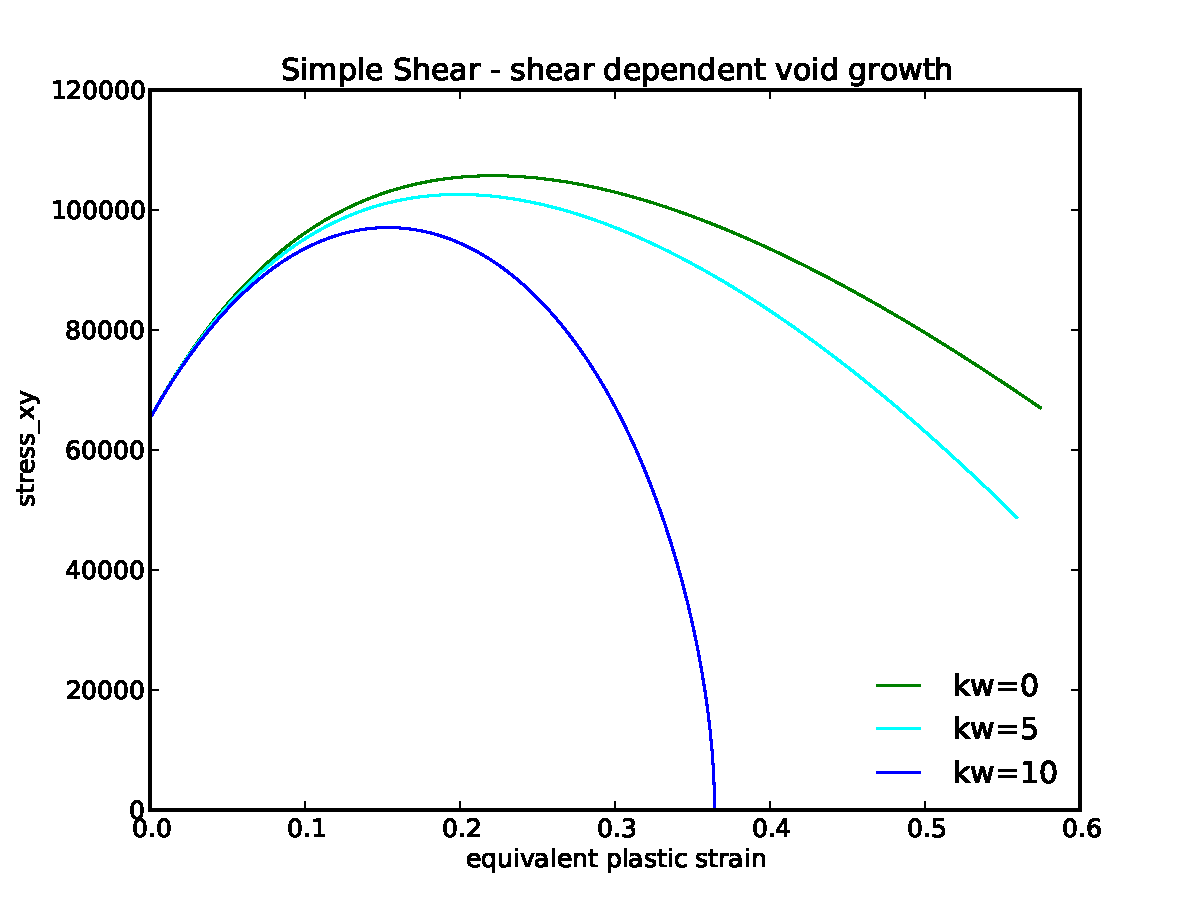
\includegraphics[trim=0mm 0mm 0mm 0
        mm,clip,width=0.5\textwidth]
      {images/stress-strain-shear-kw.pdf}}~ \subfigure[void volume
      fraction]{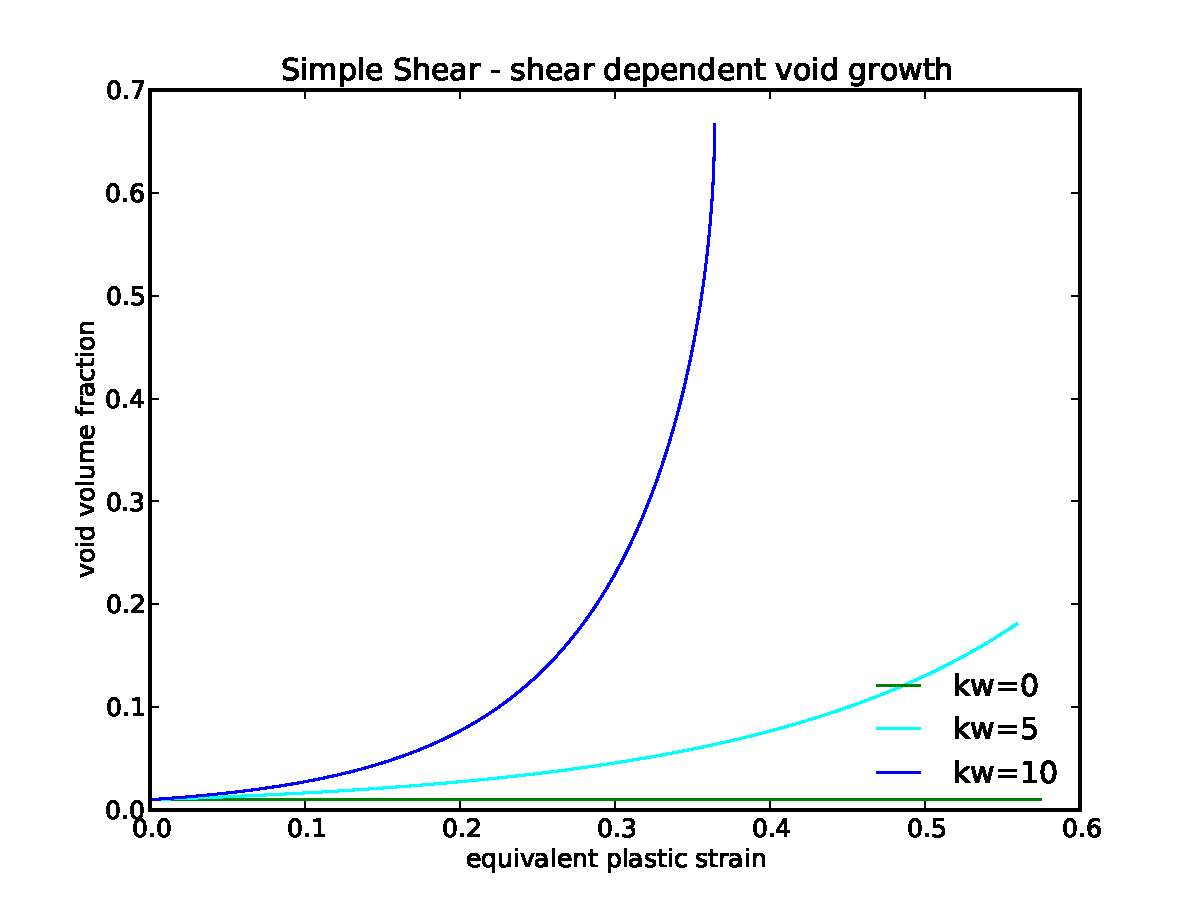
\includegraphics[trim=0mm 0mm 0mm 0
        mm,clip,width=0.5\textwidth]
      {images/void-strain-shear-kw.pdf}}
    \caption{Shear stress component and void volume fraction plotted
      against equivalent plastic strain. The shear void growth
      parameter has a pronounced effect on the response of the
      material point in simple shear.}
    \label{fig:shear-kw}
  \end{center}
\end{figure}

In Figure~\ref{fig:shear-nuc} a set of nucleation parameters are
specified and also evaluated in the simple shear scenario. In this
case the volume fraction of nucleated voids $f_{N}$, is varied, while
the mean value and standard deviation of failure strain, $\epsilon_N$
and $s_N$ respectively, are specified and held constant. Observe that
the shear stress component is somewhat reduced, to a greater extent as
the volume fraction of nucleated voids is increased. Also observe that
the void volume fraction grows by approximately the specified volume
fraction of nucleated voids, in particular, where $f_{N}$ is zero, the
void volume fraction does not deviate from zero.

\begin{figure}[htbp]
  \begin{center}
    \subfigure[stress]{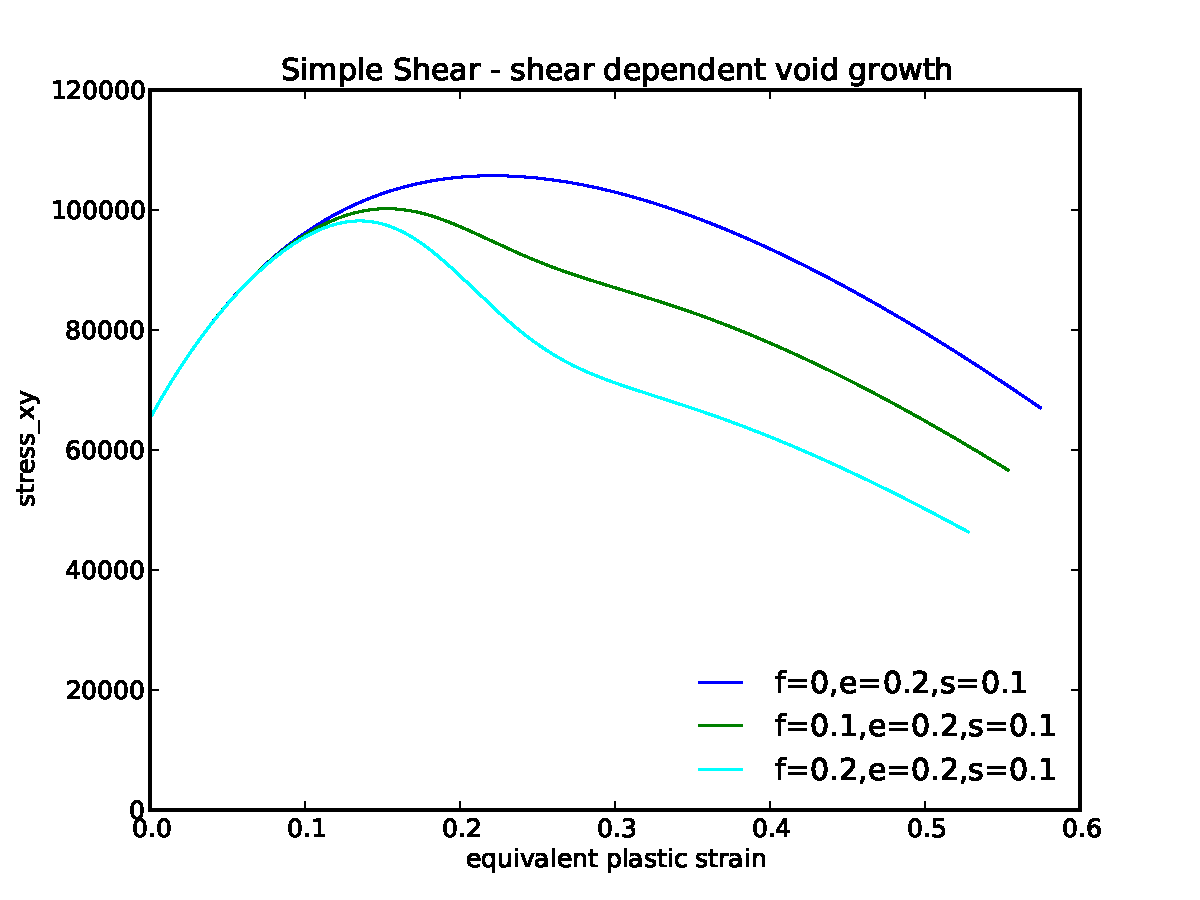
\includegraphics[trim=0mm 0mm 0mm 0
        mm,clip,width=0.5\textwidth]
      {images/stress-strain-shear-nuc.pdf}}~ \subfigure[void volume
      fraction]{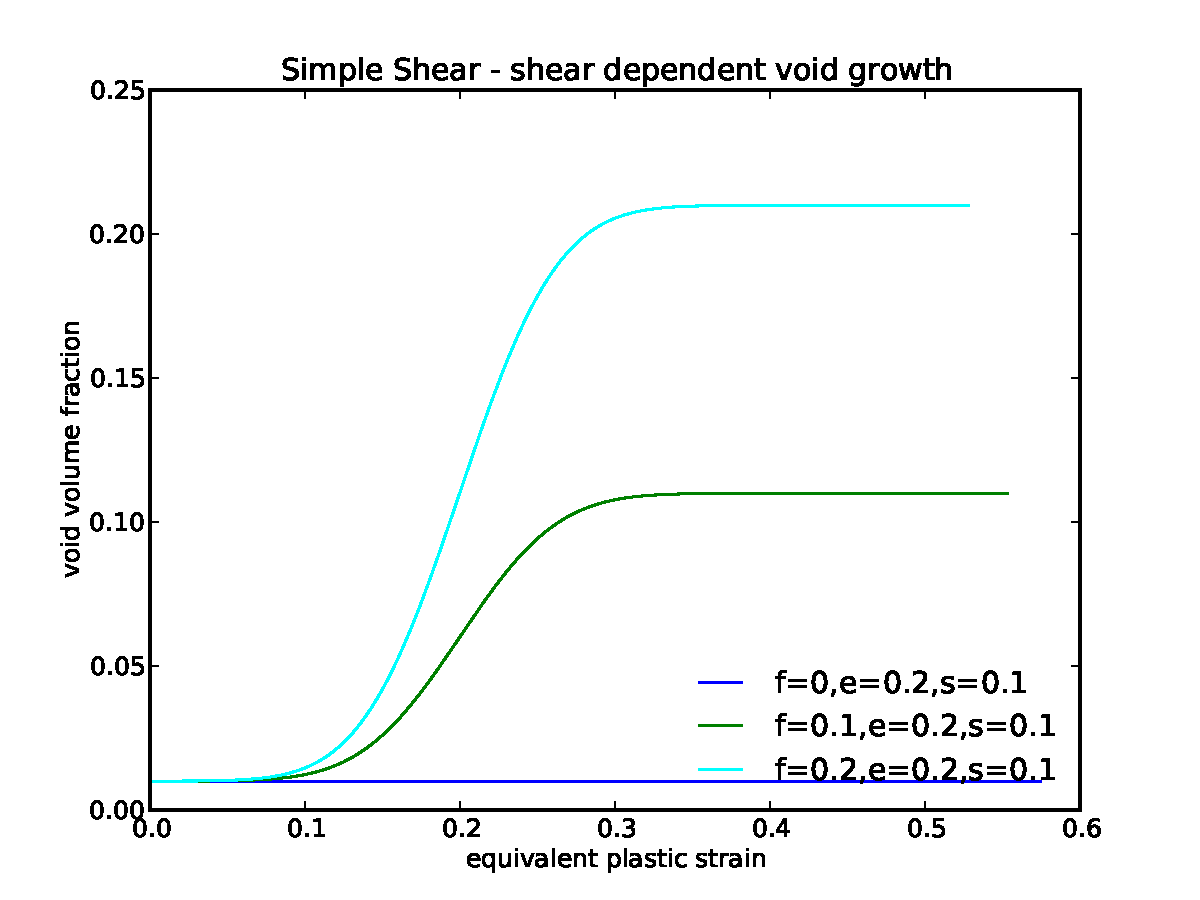
\includegraphics[trim=0mm 0mm 0mm 0
        mm,clip,width=0.5\textwidth]
      {images/void-strain-shear-nuc.pdf}}
    \caption{Shear stress component and void volume fraction plotted
      against equivalent plastic strain. The void nucleation
      parameters have some effect on the response of the
      material point in simple shear.}
    \label{fig:shear-nuc}
  \end{center}
\end{figure}

% Local Variables:
% TeX-master: "GursonModel"
% mode: latex
% mode: flyspell
% End:

    \chapter{Conclusions}
\label{conclusions}

% Local Variables:
% TeX-master: "GursonModel"
% mode: latex
% mode: flyspell
% End:


    % ---------------------------------------------------------------------- %
    % References
    %
    \clearpage
    % If hyperref is included, then \phantomsection is already defined.
    % If not, we need to define it.
    \providecommand*{\phantomsection}{}
    \phantomsection
    \addcontentsline{toc}{chapter}{References}
    %\bibliographystyle{GursonModel}
    \bibliography{GursonModel}


    % ---------------------------------------------------------------------- %
    %
    % \appendix
%     \chapter{Historical Perspective}
% 	\input{CommonHistory}


%     \chapter{Some Other Appendix}
% 	\input{CommonAppendix}

    % \printindex

    %
% This is an example of how to create the distribution page. Some
% distributions are required by Sandia; e.g. the housekeeping copies.
% Depending on the type of report; e.g. CRADA, Patent Caution, etc.
% additional distribution lines may have to be added. See the
% "Guide for Preparing SAND Reports"
%
% SANDdistribution takes CA or NM as an optional argument. If given,
% the approrpiate housekeeping copies are inserted autmatically.
% Inside the SANDdistribution environment, several commands can be used
% insert the distributions for CRADA, LDRD, etc. See example below.
%
% You can leave the CA or NM option off and not use any of the SANDdist*
% commands. This will allow you to create a distribution list manually.
%
\begin{SANDdistribution}[CA]
    % Housekeeping copies necessary for every unclassified report:
    % \SANDdistCRADA	% If this report is about CRADA work
    % \SANDdistPatent	% If this report has a Patent Caution or Patent Interest
    % \SANDdistLDRD	% If this report is about LDRD work

    % Some external Addresses
    \SANDdistExternal{1}{Qiushi Chen\\ 99 $99^{th}$ street NW\\Clemson, SC}
    \bigskip


    % The following MUST BE between the external and internal distributions!
    % \SANDdistClassified % If this report is classified


    % Internal Addresses
    \SANDdistInternal{1}{9042}{Jake Ostien}{8256}
    \SANDdistInternal{1}{9042}{James W. Foulk III}{8256}
    \SANDdistInternal{1}{????}{Kendall Pierson}{1542}

    % Example of a mail channel use (instead of a mail stop)
    %\SANDdistInternalM{1}{M9999}{Someone}{01234}

\end{SANDdistribution}


\end{document}
